% =============================================================================
% Chapitre 8 — L'univers global_2004 : un test enfin équitable
%
% Aucun chiffre de ce chapitre n'est saisi à la main. Tous proviennent des
% artefacts gelés (global_2004_readiness.json, _q1_results.json,
% _q2_results.json, _interpretation.json) et sont repris dans
% docs/GLOBAL_2004_RESULTS.md, lui-même généré.
% =============================================================================

\chapter{L'univers \texttt{global\_2004} : un test enfin équitable}
\label{chap:global2004}

Les chapitres précédents concluent qu'aucun avantage n'a été établi pour la
couche de régimes ni pour les modèles challengers. Cette conclusion souffrait
toutefois d'une faiblesse d'\emph{identification} : sur les deux univers
publiés, il n'était pas possible de distinguer « le modèle n'apporte rien » de
« le dispositif ne permet pas au modèle de s'exprimer ». Ce chapitre décrit la
construction d'un troisième univers destiné à lever cette ambiguïté, et le
résultat obtenu.

% =============================================================================
\section{Deux défauts d'identification, mesurés et non supposés}
% =============================================================================

\textbf{\texttt{etf\_2017} — la contrainte domine l'objectif.} Avec cinq actifs
et un plafond de 25~\%, la variance minimale à rétrécissement n'émet
qu'\textbf{une seule allocation distincte sur 248~rééquilibrages}.
L'arithmétique seule n'impose pas cette solution de coin — l'équipondération
demeure admissible, sans aucun actif au plafond — mais empiriquement c'est la
contrainte, et non le modèle de covariance, qui choisit le portefeuille. Une
meilleure estimation de covariance n'a alors nulle part où se manifester.

\textbf{\texttt{full\_2021} — l'entrée de covariance est biaisée.} Les séances
de Casablanca et de New York ne se recouvrent qu'à peine et les prix de la BVC
sont fréquemment figés : corrélation contemporaine de 0,0041 avec le SPY contre
0,0779 au décalage d'un jour, et 17,1~\% de journées à rendement exactement nul.
La matrice de covariance quotidienne sous-estime donc systématiquement la
dépendance entre marchés.

\begin{remarquebox}
Aucun de ces deux défauts n'est un échec de modélisation. Ce sont des propriétés
de l'\emph{ensemble d'opportunités}, ce qui explique qu'aucun changement de
modèle n'ait pu les corriger.
\end{remarquebox}

% =============================================================================
\section{Un protocole gelé avant toute donnée}
% =============================================================================

L'univers a été spécifié dans un document de pré-enregistrement
(\texttt{GLOBAL\_UNIVERSE\_PREREGISTRATION.md}) validé et \emph{horodaté par un
commit isolé} avant toute ingestion. Il fixe dix instruments cotés aux
États-Unis et libellés en dollars — \texttt{SPY}, \texttt{QQQ}, \texttt{IWM},
\texttt{EFA}, \texttt{EEM}, \texttt{IEF}, \texttt{TLT}, \texttt{LQD},
\texttt{IYR}, \texttt{GLD} — retenus par six règles d'éligibilité formulées
uniquement en attributs \emph{ex ante} : place de cotation, date de création,
catégorie de prospectus, composition déclarée. Aucune règle ne consulte un
rendement, si bien que la liste est entièrement déterminée avant qu'une seule
observation ne soit lue.

Le protocole fixe également les deux questions, leurs comparateurs, le seuil de
matérialité économique et, par amendement daté, la hiérarchie des critères
statistiques. Chaque amendement a été committé \emph{avant} le code qu'il
gouverne.

\begin{remarquebox}
Le document reconnaît lui-même ne pas être un pré-enregistrement immaculé~: des
diagnostics d'allocation avaient été inspectés avant sa rédaction et ont motivé
l'exclusion de deux instruments. Cette inspection est divulguée intégralement,
avec la précision qu'\emph{aucune grandeur de performance} n'en faisait partie.
\end{remarquebox}

% =============================================================================
\section{Le défaut d'expressivité est levé}
% =============================================================================

Avant tout calcul de performance, un point de contrôle de \emph{préparation des
données} a vérifié dix critères pré-enregistrés : fenêtre de 21,7~ans
effectivement préservée, aucune cellule reportée par remplissage avant, absence
de signature de prix figés (dominance de décalage $-0{,}0248$, exigence
$\leq 0$), et les deux garde-fous d'absence d'anticipation. Verdict~:
\textbf{READY, 10/10}.

\begin{figure}[htbp]
  \centering
  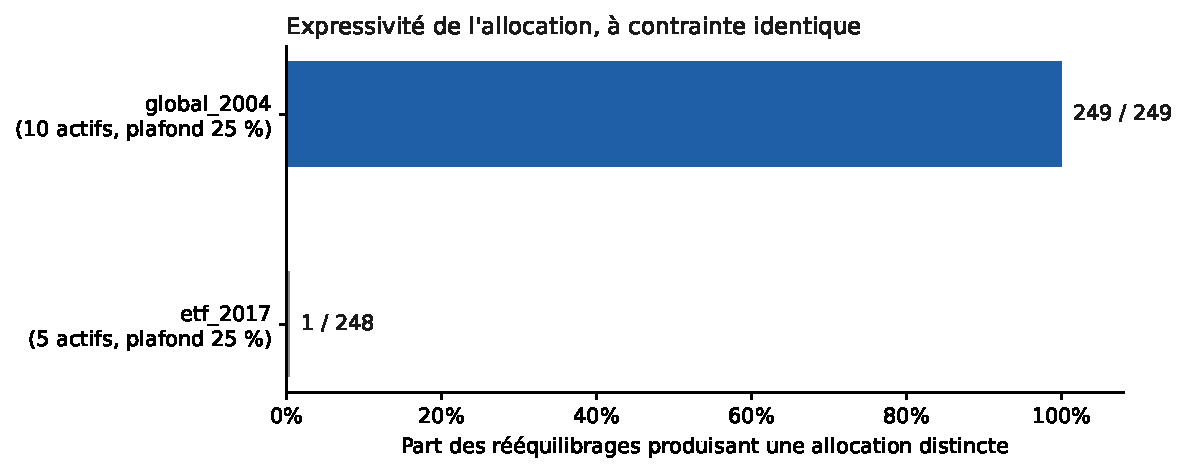
\includegraphics[width=0.92\textwidth]{assets/figures/global_2004_expressivite.pdf}
  \caption[Expressivité de l'allocation]{À contrainte strictement identique
  (plafond de 25~\%, mêmes coûts, même moteur), l'optimiseur passe d'une
  allocation unique sur 248~rééquilibrages à une allocation distincte à
  \emph{chaque} rééquilibrage. C'est la condition nécessaire pour qu'un test
  de modèle ait un sens.}
  \label{fig:g2004expressivite}
\end{figure}

% =============================================================================
\section{Q1 — la couche de régimes face au comparateur classique}
% =============================================================================

Une seule comparaison, spécifiée à l'avance, sur le segment de test gelé
(2019-01-04 à 2026-08-14, 1\,913~jours)~: \texttt{regime\_conditional} contre
\texttt{max\_sharpe}, nette de coûts. Aucune correction de tests multiples n'est
appliquée, car une hypothèse unique fixée d'avance n'en requiert pas.

Le Sharpe net observé est de \textbf{0,8923} pour la stratégie à régimes contre
\textbf{0,9785} pour le comparateur, soit un écart de $-0{,}0862$ avec un
intervalle à 90~\% de $[-0{,}2133;\ +0{,}0414]$ et une valeur~$p$ unilatérale de
$0{,}8596$. Les deux verdicts pré-enregistrés sont négatifs.

Trois lectures que le seul ratio de Sharpe masquerait~:

\begin{itemize}
  \item \textbf{Les coûts n'ont pas créé le résultat.} Le Sharpe \emph{brut}
        était déjà inférieur ($0{,}9080$ contre $0{,}9820$)~: il ne s'agit pas
        d'un signal informatif annulé par les frictions de transaction.
  \item \textbf{La rotation est 4,3 fois supérieure} ($0{,}1224$ contre
        $0{,}0285$).
  \item \textbf{La stratégie à régimes ne perd pas sur toutes les dimensions}~:
        sa perte maximale est \emph{moindre} ($-24{,}22~\%$ contre
        $-25{,}27~\%$).
\end{itemize}

\begin{remarquebox}
En résultat secondaire, l'intervalle apparié pour la différence de rendement
moyen annualisé est entièrement négatif. Il serait donc inexact de résumer Q1
par « aucune différence établie » sans qualification~: c'est vrai de la
comparaison en Sharpe, qui est la question enregistrée, et faux de cet
intervalle.
\end{remarquebox}

% =============================================================================
\section{Q2 — la famille des challengers, et la correction}
% =============================================================================

Q2 est une \emph{recherche} et non une comparaison unique~: les
\textbf{240~configurations atteignables} (grilles d'hyperparamètres
RF/XGBoost croisées avec les leviers de construction de portefeuille) ont toutes
été évaluées, sans qu'aucune ne soit écartée sur la base de sa performance
observée. L'hypothèse nulle testée est composite~: \emph{aucun} candidat de la
famille ne surperforme la référence.

\begin{figure}[htbp]
  \centering
  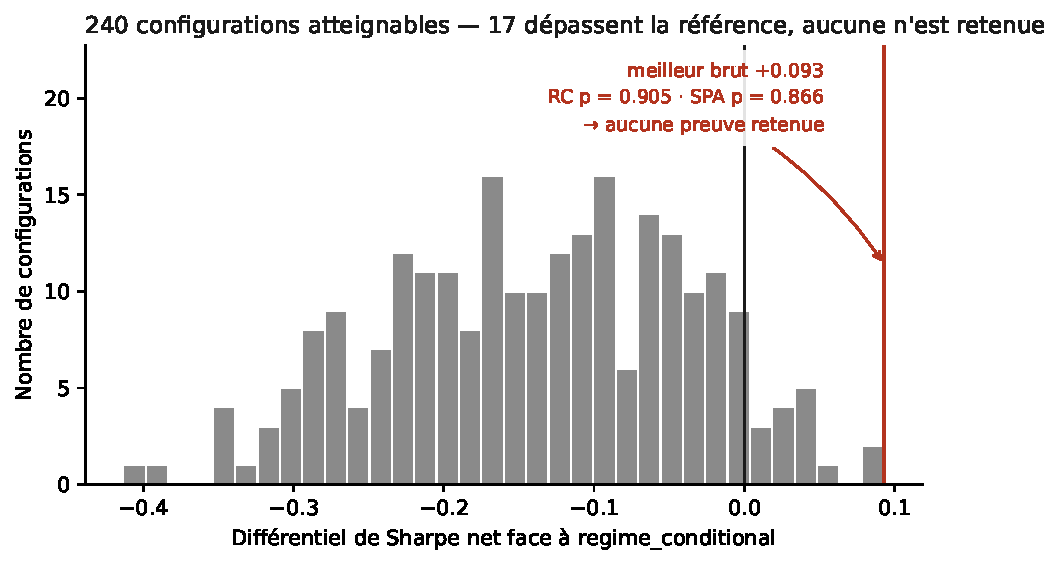
\includegraphics[width=0.94\textwidth]{assets/figures/global_2004_correction.pdf}
  \caption[Correction pour tests multiples]{Distribution des 240~différentiels
  de Sharpe face à \texttt{regime\_conditional}. Le meilleur candidat brut
  dépasse la référence de $+0{,}093$ — davantage, en valeur absolue, que
  l'écart de Q1 et en sens inverse. Les tests de White et de Hansen refusent
  cette valeur~: elle est le maximum d'une recherche de 240~configurations, et
  c'est précisément ce que la correction facture.}
  \label{fig:g2004correction}
\end{figure}

Sur le critère \textbf{primaire} (différentiel de Sharpe), le Reality Check de
White donne $p = 0{,}905$ et le SPA de Hansen $p = 0{,}866$~; sur le critère
secondaire, $0{,}457$ et $0{,}358$. Aucun test ne rejette sur aucun critère~:
\texttt{concordant\_evidence\_of\_family\_outperformance} vaut \textbf{faux}.
Seules 17~des 240~configurations dépassent la référence en Sharpe.

% =============================================================================
\section{Les challengers honnêtement sélectionnés}
% =============================================================================

La valeur~$p$ de la famille répond à la question « le meilleur des 240 est-il
crédible~? ». Une question différente, et plus proche de la pratique, est
« qu'aurait obtenu un praticien discipliné~? ». Les configurations retenues par
une sélection \emph{strictement antérieure} — validation croisée à fenêtre
glissante avant, puis choix des leviers sur le segment de validation, le
segment de test n'étant jamais montré à un sélecteur — donnent~:

\begin{figure}[htbp]
  \centering
  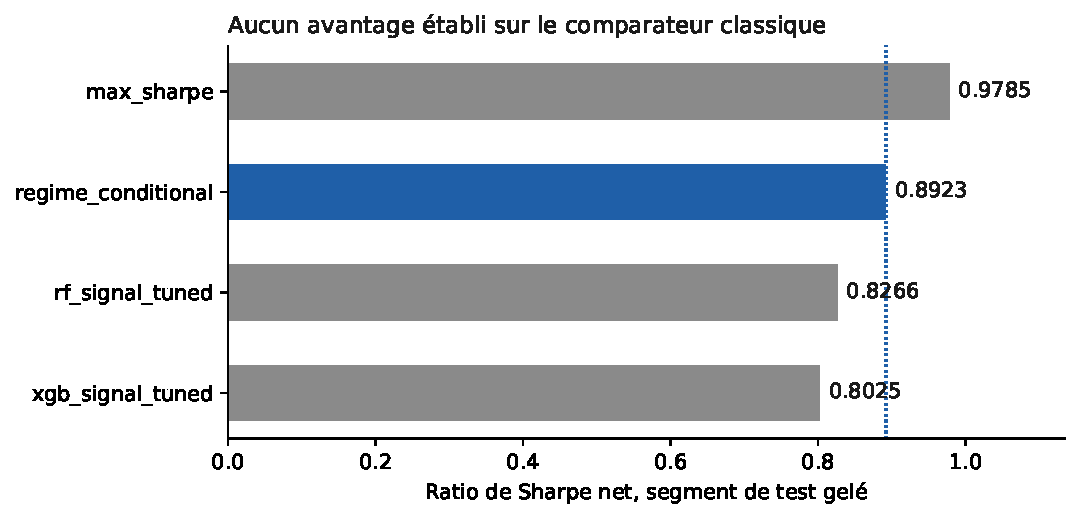
\includegraphics[width=0.92\textwidth]{assets/figures/global_2004_sharpes.pdf}
  \caption[Sharpe des stratégies retenues]{Sharpe net \emph{observé} sur le
  segment de test gelé. Les deux challengers honnêtement sélectionnés y
  affichent une valeur inférieure à celle de la stratégie à régimes,
  elle-même inférieure à celle du comparateur classique. Aucun test pairé
  individuel n'a été pré-spécifié pour ces écarts~: ce sont des grandeurs
  descriptives.}
  \label{fig:g2004sharpes}
\end{figure}

Les challengers RF et XGBoost honnêtement sélectionnés affichent un Sharpe net
observé inférieur de respectivement $0{,}0657$ et $0{,}0898$ à celui de
\texttt{regime\_conditional}. Ce constat descriptif est pertinent pour la
sélection opérationnelle, mais ne constitue pas une preuve statistique de
sous-performance~: \textbf{aucun test pairé individuel de ces écarts n'a été
pré-spécifié}.

C'est donc un \emph{diagnostic opérationnel complémentaire} du verdict de
famille, et non une version plus forte de celui-ci~: le test de famille demande
si le meilleur de 240 est crédible, tandis que ce constat décrit ce qu'un
praticien discipliné aurait effectivement détenu.

\textbf{Ce résultat n'est pas un artefact de repli.} La télémétrie enregistre
\emph{un} repli sur 59\,760~ajustements de la famille, trois sur 249 pour la
référence — tous antérieurs au segment de test — et \textbf{zéro} pour les deux
challengers sélectionnés. Chaque chiffre provient donc du modèle que son
étiquette désigne.

% =============================================================================
\section{Limites}
% =============================================================================

\textbf{Ces évaluations ne sont pas indépendantes.} \texttt{etf\_2017} et
\texttt{global\_2004} partagent cinq instruments (\texttt{SPY}, \texttt{QQQ},
\texttt{EEM}, \texttt{GLD}, \texttt{TLT}) et des périodes d'évaluation qui se
recouvrent largement~; elles subissent donc les mêmes chocs de marché. Il faut
les décrire comme \textbf{deux évaluations distinctes mais statistiquement
recouvrantes}, jamais comme des confirmations indépendantes.

\textbf{Attribution.} Q2 modifie deux choses à la fois par rapport aux univers
publiés~: la coupe transversale d'actifs \emph{et} la politique de variables
macroéconomiques (le bloc Bank Al-Maghrib est exclu, l'univers étant en
dollars). Les challengers consommant des variables macro, leurs résultats ne
peuvent pas être attribués au seul élargissement de l'univers. Q1 échappe à ce
biais, aucune de ses deux stratégies ne lisant de colonne macro.

\textbf{Sélection externe résiduelle.} Les corrections de White et de Hansen
portent sur la recherche de \emph{stratégies}. Rien ne corrige la décision, en
amont, de \emph{construire} \texttt{global\_2004} après avoir constaté que les
deux univers publiés étaient chacun défectueux.

\begin{remarquebox}
\textbf{Conclusion autorisée.} Le plafond de 25~\% rendait \texttt{etf\_2017}
faible pour l'attribution de modèle. Une fois l'expressivité de l'allocation
rétablie dans \texttt{global\_2004}, aucun avantage de la couche de régimes ni
des challengers n'a davantage été établi. La domination du plafond n'était donc
pas la seule explication du résultat négatif antérieur.
\end{remarquebox}

\texttt{global\_2004} demeure une \textbf{expérience de recherche}~: il n'est
raccordé ni à l'interface REST, ni au tableau de bord, ni à aucune allocation
destinée à la production, et aucun résultat publié n'en dépend.
